\documentclass[tikz,border=6pt]{standalone}
\usepackage{amsmath,amssymb}
\usepackage{xcolor}
\definecolor{accent}{HTML}{A13D2C}
\definecolor{accent2}{HTML}{2B5F6B}
\definecolor{muted}{HTML}{5A564F}
\definecolor{panel}{HTML}{F8F6F0}
\definecolor{linecol}{HTML}{D8D2C4}
\definecolor{astroblue}{HTML}{1B4F72}
\definecolor{ink}{HTML}{1E1C1A}
\usetikzlibrary{calc,arrows.meta}
\usepackage{pgfplots}\pgfplotsset{compat=1.18}
\usepackage[T1]{fontenc}\usepackage{newpxtext,newpxmath}  % same fonts as the notes
\begin{document}
% What D does in the sampling argument (Section "The Nyquist Sampling Criterion").
% (a) round mirror of diameter D and a copy shifted by lambda u; the overlap area sets the
%     strength of the ripple with u cycles per radian (Eq. re:eq:band_limit).
% (b) that overlap against u, for a star: (2/pi)[acos x - x sqrt(1-x^2)], x = lambda u / D, zero at u = D/lambda.
% (c),(d) the spectrum of the sampled image: copies of (b) every 1/theta_pix (Eq. re:eq:sampled_spectrum),
%     with 1/theta_pix = 2.6 D/lambda (fine pixels) and 1.45 D/lambda (coarse pixels). Frequencies in units of D/lambda.
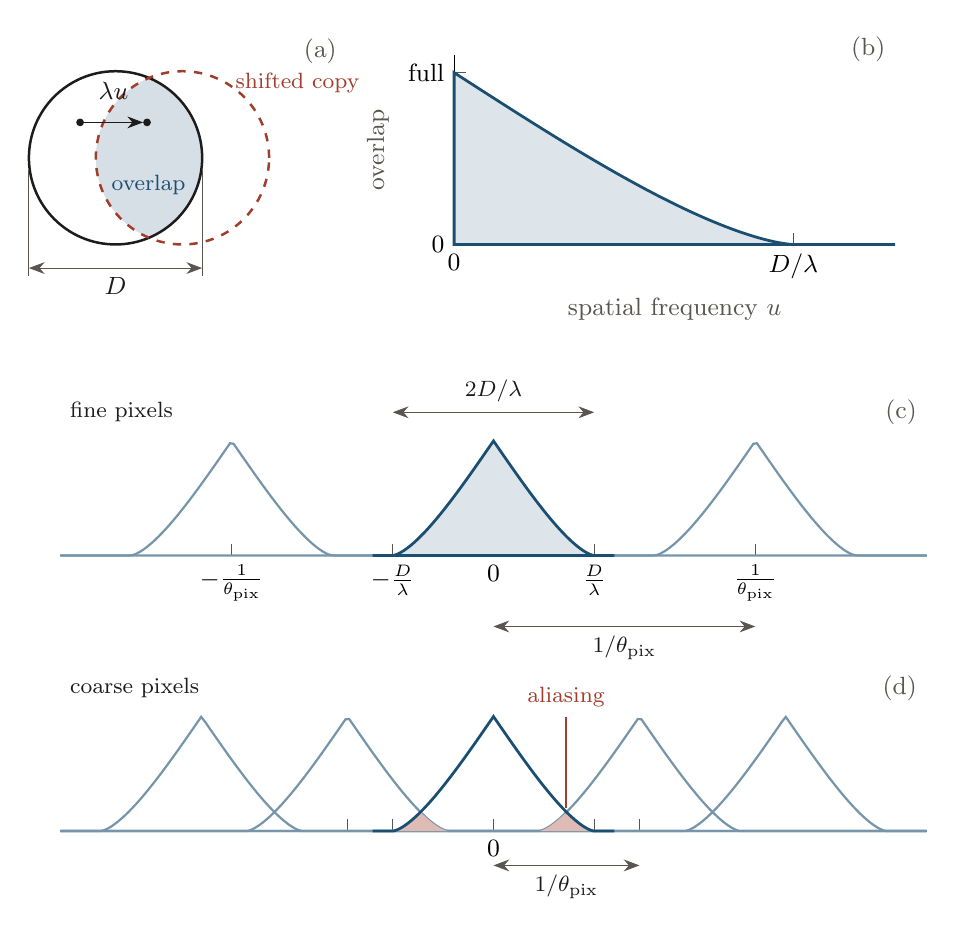
\begin{tikzpicture}[font=\small, >={Stealth[length=2mm]},
  declare function={ov(\x)=(abs(\x)<1) ? (2/pi)*(rad(acos(min(abs(\x),1)))-abs(\x)*sqrt(max(1-\x*\x,0))) : 0;}]
  \pgfplotsset{every axis/.append style={scale only axis, axis lines*=left, tick style={muted},
      every axis label/.style={text=muted}, clip=false, samples=241}}
  % (a) the mirror and its shifted copy
  \begin{scope}[shift={(1.3,1.45)}]
    \def\R{1.1}\def\s{0.85}
    \begin{scope}\clip (0,0) circle (\R); \fill[astroblue!18] (\s,0) circle (\R);\end{scope}
    \draw[ink, line width=0.9pt] (0,0) circle (\R);
    \draw[accent, dashed, line width=0.9pt] (\s,0) circle (\R);
    \draw[<->, muted] (-\R,-\R-0.3) -- node[below, ink] {$D$} (\R,-\R-0.3);
    \draw[muted] (-\R,-0.15) -- (-\R,-\R-0.4) (\R,-0.15) -- (\R,-\R-0.4);
    \fill[ink] (-0.45,0.45) circle (1.4pt); \fill[ink] (-0.45+\s,0.45) circle (1.4pt);
    \draw[->, ink] (-0.4,0.45) -- (-0.5+\s,0.45); \node[ink, anchor=south] at (-0.45+0.5*\s,0.62) {$\lambda u$};
    \node[astroblue, font=\footnotesize] at (0.42,-0.35) {overlap};
    \node[accent, anchor=west, font=\footnotesize] at (\s+0.55,0.95) {shifted copy};
    \node[muted] at (2.6,1.35) {(a)};
  \end{scope}
  % (b) overlap against u
  \begin{axis}[name=b, at={(5.6cm,0.35cm)}, width=5.6cm, height=2.4cm, xmin=0, xmax=1.3, ymin=0, ymax=1.1,
      xtick={0,1}, xticklabels={0,$D/\lambda$}, ytick={0,1}, yticklabels={0,full},
      xlabel={spatial frequency $u$}, ylabel={overlap}]
    \addplot[astroblue, line width=1pt, fill=astroblue!15, domain=0:1.3] {ov(x)} \closedcycle;
    \node[muted, anchor=north east] at (rel axis cs:1,1.15) {(b)};
  \end{axis}
  % (c) fine pixels: copies apart
  \begin{axis}[name=c, at={(0.6cm,-3.6cm)}, width=11cm, height=1.6cm, xmin=-4.3, xmax=4.3, ymin=0, ymax=1.1,
      axis y line=none, xtick={-2.6,-1,0,1,2.6}, xticklabels={$-\tfrac{1}{\theta_{\rm pix}}$,$-\tfrac{D}{\lambda}$,0,$\tfrac{D}{\lambda}$,$\tfrac{1}{\theta_{\rm pix}}$}]
    \pgfplotsinvokeforeach{-1,1}{\addplot[astroblue!60, line width=0.8pt, domain=-4.3:4.3] {ov(x-#1*2.6)};}
    \addplot[astroblue, line width=1pt, fill=astroblue!15, domain=-1.2:1.2] {ov(x)} \closedcycle;
    \draw[<->, muted] (axis cs:-1,1.25) -- node[above, ink, font=\footnotesize] {$2D/\lambda$} (axis cs:1,1.25);
    \draw[<->, muted] (axis cs:0,-0.62) -- node[below, ink, font=\footnotesize] {$1/\theta_{\rm pix}$} (axis cs:2.6,-0.62);
    \node[ink, anchor=west, font=\footnotesize] at (axis cs:-4.3,1.25) {fine pixels};
    \node[muted, anchor=east] at (axis cs:4.3,1.25) {(c)};
  \end{axis}
  % (d) coarse pixels: copies overlap
  \begin{axis}[name=d, at={(0.6cm,-7.1cm)}, width=11cm, height=1.6cm, xmin=-4.3, xmax=4.3, ymin=0, ymax=1.1,
      axis y line=none, xtick={-1.45,-1,0,1,1.45}, xticklabels={,,0,,}]
    \pgfplotsinvokeforeach{-2,2}{\addplot[astroblue!60, line width=0.8pt, domain=-4.3:4.3] {ov(x-#1*1.45)};}
    \pgfplotsinvokeforeach{-1,1}{\addplot[astroblue!60, line width=0.8pt, domain=-4.3:4.3] {ov(x-#1*1.45)};}
    \addplot[accent, fill=accent!35, draw=none, domain=0.45:1] {min(ov(x),ov(x-1.45))} \closedcycle;
    \addplot[accent, fill=accent!35, draw=none, domain=-1:-0.45] {min(ov(x),ov(x+1.45))} \closedcycle;
    \addplot[astroblue, line width=1pt, domain=-1.2:1.2] {ov(x)};
    \draw[<->, muted] (axis cs:0,-0.3) -- node[below, ink, font=\footnotesize] {$1/\theta_{\rm pix}$} (axis cs:1.45,-0.3);
    \node[accent, anchor=south, font=\footnotesize] at (axis cs:0.72,1.0) {aliasing};
    \draw[accent] (axis cs:0.72,1.0) -- (axis cs:0.72,0.2);
    \node[ink, anchor=west, font=\footnotesize] at (axis cs:-4.3,1.25) {coarse pixels};
    \node[muted, anchor=east] at (axis cs:4.3,1.25) {(d)};
  \end{axis}
\end{tikzpicture}
\end{document}
